\documentclass[tikz]{standalone}

\newcommand{\pt}[3]{\fill[#3] (#1,#2) circle (1.7pt);}

\begin{document}
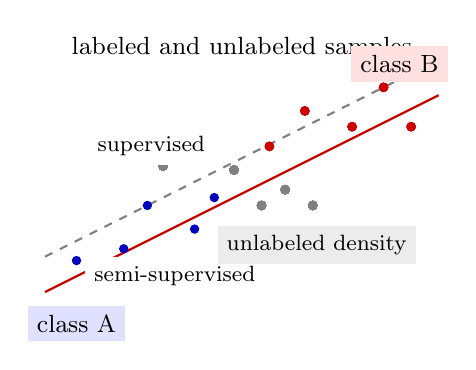
\begin{tikzpicture}[font=\small]
  \node at (2.9,3.25) {labeled and unlabeled samples};
  \draw[gray,dashed,thick] (.4,.6) -- (5.4,3.1);
  \draw[red!80!black,thick] (.4,.15) -- (5.4,2.65);
  \foreach \x/\y in {.8/.55,1.4/.7,1.7/1.25,2.3/.95,2.55/1.35} \pt{\x}{\y}{blue!75!black}
  \foreach \x/\y in {3.25/2,3.7/2.45,4.3/2.25,4.7/2.75,5.05/2.25} \pt{\x}{\y}{red!80!black}
  \foreach \x/\y in {1.9/1.75,2.35/1.85,2.8/1.7,3.15/1.25,3.45/1.45,3.8/1.25} \pt{\x}{\y}{gray}
  \node[fill=blue!12] at (.8,-.25) {class A};
  \node[fill=red!12] at (4.9,3.05) {class B};
  \node[fill=white,font=\footnotesize] at (1.75,2) {supervised};
  \node[fill=white,font=\footnotesize] at (2.05,.35) {semi-supervised};
  \node[fill=gray!15,font=\footnotesize] at (3.85,.75) {unlabeled density};
\end{tikzpicture}
\end{document}
